\documentclass[12pt, letterpaper, twocolumn, titlepage]{article}

%package imports
\usepackage[compact]{titlesec}
\usepackage{fullpage}              %for margins
\usepackage{setspace}              %line spacing
\usepackage{fancyhdr}              %headers
\usepackage{wrapfig}
\usepackage{graphicx}
\usepackage{float}

%page layout setup
\setlength{\headheight}{14.5pt}
\setlength{\headsep}{25pt}

%header setup
\pagestyle{fancyplain}
\fancyhf{}

\lhead{\fancyplain{}{\textsc{2013 RoboSub Competition}}}     %top left
\chead{\fancyplain{}{}}	                    %top center
\rhead{\fancyplain{}{\textsc{Journal Paper}}}         %top right
\lfoot{\fancyplain{}{\textsc{St.~George's Robotics Team}}}	                    %bottom left
\cfoot{\fancyplain{}{}}       %bottom center
\rfoot{\fancyplain{}{\thepage}}                     %bottom right

\renewcommand{\headrulewidth}{0pt}
\renewcommand{\footrulewidth}{0pt}

\newcommand{\CPP}
{C\nolinebreak[4]\hspace{-.05em}\raisebox{.22ex}{\footnotesize\bf ++}}

\setlength{\parskip}{1mm plus0mm minus0mm}

\titlespacing*{\section}{0pt}{3ex}{1ex}
\titlespacing*{\subsection}{0pt}{2.5ex}{0ex}
\titlespacing*{\subsubsection}{0pt}{2ex}{0ex}

%document beginning
\begin{document}

%title
\title{\vspace{-10pc}
\includegraphics{Logo.png}\\\vspace{2pc}\textsc{St.\ George's Robotics Team}\\
\LARGE{Autonomous Underwater Vehicle}}
\author{Spencer Chan\\Calvin Cheng\\Stanley Cho\\Evan Johnson\\Spencer Louie\\Ezaan Mangalji\\Giulio Rossi\\Marcus Tan\\Kevin Tian\\Raymond Wang\\Carl Xi\\Leon Zhou}
\date{AUVSI Foundation and ONR's\\16th International RoboSub Competition\\SSC Pacific TRANSDEC, San Diego, CA\\July 22--28, 2013}
\maketitle

\setstretch{1.1}
\setlength{\columnsep}{1.4pc}

\begin{abstract}
Following a successful showing at the 2009 AUVSI RoboSub Competition, the St.\ George's Robotics Team has built a new autonomous underwater vehicle from scratch, which it is proud to enter into 2013 competition. The design of the robot is built around the general architecture of a dirigible airship; the main computer and batteries are located in a long cylindrical tube, with the ``gondola'' section of the robot housing the thrusters and propulsion system.

The sensors attached to the system include an accelerometer, a gyroscope, a compass, a pressure (depth) sensor, and a Hall effect sensor, which will work in coordination with a Dreamplug computer to control the movement and direction of the AUV.

Needless to say, the robot this year is merely a skeleton of what the team hopes to accomplish in the upcoming years; the plan for competition this year will be more of a learning experience to see what can be improved upon in the future, in terms of both hardware and software. This is also the first time competing in the RoboSub competition for all of the team members; regardless, despite the lack of experience, the team hopes to remain competitive in the field with this autonomous underwater vehicle, which has taken the team three years to meticulously build and put together.
\end{abstract}


\section{Introduction}

\subsection{Team Background}
St.~George's School is a high school located in Vancouver, BC. Although the school is known for its myriad athletic, artistic, and academic pursuits, one area from which little is often heard is its robotics program. In 2009, the St.~George's Robotics team competed in the RoboSub Competition for the first time in school history, finishing 17th in the competition, and earning the ``Best New Team'' award. As the participants in competition are primarily prestigious universities, this finish was quite an accomplishment for the Saints team.

Robotics at St.~George's has always existed an entirely extra-curricular endeavour; the members of the robotics team do research, plan collaboratively, and construct the robot all outside of class time. The team that is participating in the competition this year is a completely new crew from the 2009 team, as all of the members of the former team have graduated. The robot has also been built entirely from scratch: the philosophy of the team is that once all the members who took part in the initial construction of the robot have departed, that robot must be retired.

This current robot has taken three years to finally take shape. Unlike a number of other teams in the competition, the St.~George's Robotics team runs on a very restricted budget; the funding to the robotics program has been fairly limited over the past few years. As a result, the team has opted to save money over time as much as possible, resulting in a much lengthier time required to construct this AUV. Build sessions have typically occurred on Sunday afternoons, after school on weekdays, and during holiday breaks.

The robotics team is divided roughly into three general groups. One part of the team focuses on the mechanical aspects of the robot, using lathes, drill presses, and saws among other tools in order to craft the variety of pieces required for this complex machine. The second group, the programmers, work intensely with the sensors and the computer in order to create an interface that will allow the robot to complete the course with the least margin of error possible.

Finally, a number of members work on communicating information, not only between the former two groups, but to the general public as to the progress of the robot. This group comprises the photographers, video producers, website designers, and report writers. Needless to say, cooperation between these groups was essential to the success of the robot, so the team was very fortunate to comprise members who were so willing to work together to ensure that the AUV was built as efficiently and economically as possible.

\subsection{Robot Design}
This AUV is based of the general structure of a standard dirigible airship. Though the base elements were inspired by the robot crafted by the team of 2009, a number of improvements have been added to address the shortcomings of the previous design.

The main systems are housed inside a cylindrical acrylic tube, inside which the battery compartments and main computer are stored. At one end of the tube is the compass, and at the other end, an aluminium end cap to dissipate the heat generated by the computer within the module.

Waterproof wires lead from the end cap into a thruster under an aluminium frame suspended under the main tube. This thruster turns a brass rod, which is attached to a worm gear. As the worm gear connects to the thrusters on either side of the robot, sending a signal to power the central thruster (which results in the revolution of the worm gear) will cause the vertical angle of the forward thrusters on either side to change. This is how the depth of the robot will be controlled; the powering of the two thrusters on either side when they are tilted upwards will cause the AUV to rise, and tilting them downwards will cause the opposite to occur.

\subsection{Mission Strategy}
The principal goal this year is fairly simple: to pass through the validation gate, follow the path, and finish up at the traffic light buoys. Based on the limited equipment/sensors available on board the AUV this year, this seems to be the most realistic estimate of the number of tasks that can be completed.

Although the number of tasks completed seems to be small, the team also hopes to gain a number of points via subjective measures, such as the quality of the team website, journal paper, and introductory video. Because every member of the team is quite knowledgeable about the design rationale behind most of the decisions made during the construction of this AUV, the team also hopes to gain points simply through their knowledge of the inner workings of the robot during the static judging stage.

\section{Hardware}

The hardware aspect of the AUV can be roughly categorized into two main sections: the mechanical portion, which includes all of the metals, plastics, and other materials used to construct the skeleton of the robot, and the electrical portion, which comprises all of the onboard sensors, computers, and controllers used to navigate the AUV throughout the course.

\subsection{Mechanical}

The major mechanical parts of the AUV—the battery compartments and the computer—are enclosed in the main housing. Below the main housing lie the parts needed for the operation of the three thrusters, which are used to control the propulsion and orientation of the robot.

\subsubsection{Hull}

The central components of the robot are housed inside an acrylic cylindrical tube, 3 feet in length with an 5.25-inch inner diameter and a 5.5-inch outer diameter. The team opted for acrylic primarily because the material is transparent, making more apparent any leaks and any other issues issues in the water. Acrylic is also quite durable, an important quality considering that the tube houses the most critical parts of the robot.

The end cap of the tube is crafted from aluminium, selected for its heat conductivity and malleability. These properties reduced the time required to machine the end cap down to size and made it easier to fit the O-rings and waterproof wires into the end cap; furthermore, they allow for effective heat dissapation away from the computer mounted to the end cap during the actual operation of the robot.

Below the cylindrical tube is an aluminium frame which was used to hold the thrusters in place. Again, aluminium was chosen due to its durability and relatively low cost. Because the frame will be immersed in water, the frame was anodized to prevent corrosion and to increase surface hardness. In order to prevent the aluminium frame from scratching the acrylic tube, a foam cushion lies in between the frame and the tube. The foam was coated in fiberglass, to prevent the foam from chipping away in transport and to preserve its form when submerged.

\subsubsection{Battery Compartments}

Within the acrylic tube lies the battery holders. Much time was taken to ensure that the battery holders were built properly, as they would occupy the largest amount of space within the tube.

\begin{wrapfigure}{r}{0.38\columnwidth}
	\vspace{-30pt}
 	\flushright
   	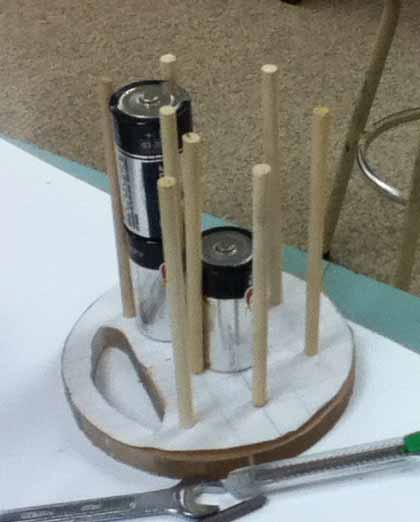
\includegraphics[width=0.38\columnwidth]{Battery}
   	\vspace{-30pt}
\end{wrapfigure}

Acrylic was the material of choice, due its strength and transparency. A total of 14.4 volts were needed to power the entire robot, so the usage of 12 D-size batteries ($1.2$\,V each) in series was decided upon, to ensure that sufficient power was available to the robot. A lathe was used to machine the half-inch sheet of acrylic into a circle, just enough for it to friction-fit into the cylindrical housing. Indents were drilled at various points into the acrylic to fit brass rods---these rods would be used to connect the two ends the battery holder, eventually compressing the batteries within.

A relatively large hole was also drilled into the top of the material where no batteries would be placed, for two reasons. The hole lessens the weight of the robot, an important consideration as the weight of the robot is factored in during the competition. In addition, as the battery holder spans the entire interior width of the central housing, space was needed for the wires to pass through; the hole accomplishes just that.

\subsubsection{Thrusters}

\begin{wrapfigure}{r}{0.29\columnwidth}
	\vspace{-30pt}
 	\flushright
   	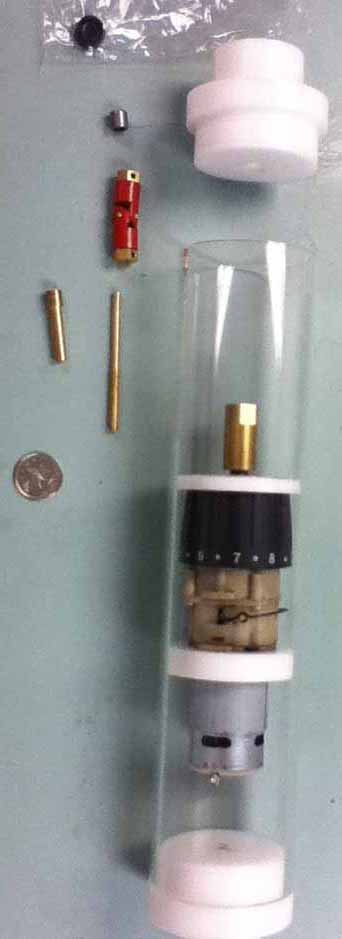
\includegraphics[width=0.29\columnwidth]{Thrusters}
   	\vspace{-30pt}
\end{wrapfigure}

The thrusters took perhaps the longest time to machine, as the budget did not allow for commercially-made thrusters to be purchased. Yet again, acrylic was the material of choice for the tube, as its transparent, lightweight, and cost-effective qualities was ideal. The end caps were made of acetal, due to its machinability; as the team did not have access to large industrial power tools, ease of machining was a large factor in determining materials used.

\noindent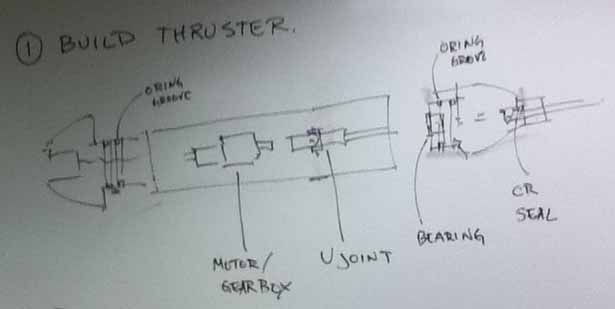
\includegraphics[width=\columnwidth]{ThrusterDesign}\vspace{-8pt}\\

To further cut costs, the motors in all three thrusters were taken from old, unused hand drills and were machined to fit into the acrylic tubes. Each motor is connected to the end cap with a rod. However, as the thrusters will be placed in water and will thus encounter a significant amount of resistance, U-joints were placed on the rods to allow for vibration from outside without damaging the motors.

Propellers were fitted onto the end of two of the thrusters; the final thruster was connected to a worm gear that would allow the other two thrusters to adjust their vertical angle. On the other end of the three thrusters, the power supply was attached; waterproof wire connections were crucial here, which will be described more in depth in a later section. The wires brought power to the motor, which allowed the robot to run in the water.

\subsection{Electrical}

The electrical components of the AUV followed a similar thought process as that of the mechanical components---if a component had to be purchased, the cheapest one that provided the bare necessary utility was selected.

\subsubsection{Computer}

The computer on board the AUV is a DreamPlug system with a Marvell\textregistered{} Sheeva\texttrademark{} Core embedded processor at 1.2 GHz, 4 GB of on-board flash memory, and 512 MB of 16-bit DDR2 SDRAM.\\

\noindent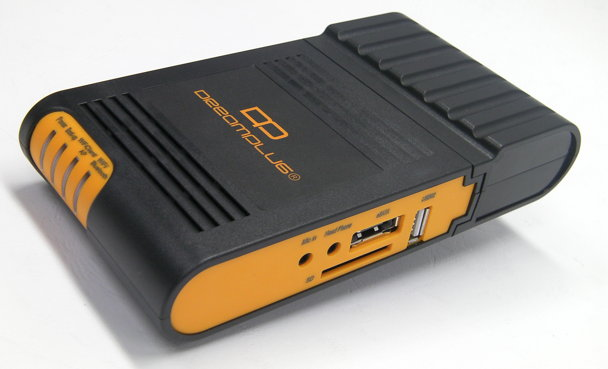
\includegraphics[width=\columnwidth]{Dreamplug}

This computer was chosen over other viable systems such as a Raspberry Pi due to its lower cost and power consumption; even under maximum processing load, the system draws only 5 volts and 3 amps of power.

In addition, because the system has several ports and connections, including 2 USB ports, 2 Gigabit Ethernet ports, an SD card slot, and WiFi connectivity, this computer was quite effective at delivering all of the necessary input and output through the various ports, despite the limited processing power. The small form factor of this computer also allowed for more space in the main housing, as well as less weight.

Consideration was also given to the level of heat generated by the computer; in fact, one of the reasons this DreamPlug was chosen over more powerful computers is that it would generate less heat. During the team's previous appearance at the competition, overheating was a major problem; consequently, one of the major focuses this year in the design was minimizing heat-related issues. To this end, the computer inside the main housing will be mounted to the aluminium end cap, which will ideally serve as a heat sink and dispel as much heat as possible into the water.

\subsubsection{Wiring}

Given that the AUV will be fully submerged, it was imperative that all of the
\begin{wrapfigure}{r}{0.28\columnwidth}
	\vspace{-30pt}
 	\flushright
   	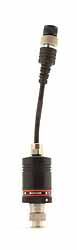
\includegraphics[width=0.28\columnwidth]{Wiring}
   	\vspace{-50pt}
\end{wrapfigure}
electrical components were protected from shorting out due to contact with water. Although the original idea was to machine waterproof wire connections in-house, the team soon discovered that the precision required to create a waterpoof seal was not feasible with the equipment available. As a result, the team decided to purchase and use Ikelite ICS underwater connectors for the many areas on the AUV that require a waterproof seal around the wire. While somewhat costly, this provided much-needed peace of mind for the most vulnerable parts of the robot.

\subsubsection{Motor Control}

The two main modules that affected the control of the motors consisted of the servo controller and Hall effect sensor, both which allowed the robot fine control of the position of the motors at all times.

\paragraph{Servo Controller}

A Phidget Advanced Servo Controller was used to control the movement of the motors. Through
\begin{wrapfigure}{r}{0.4\columnwidth}
	\vspace{-30pt}
 	\flushright
   	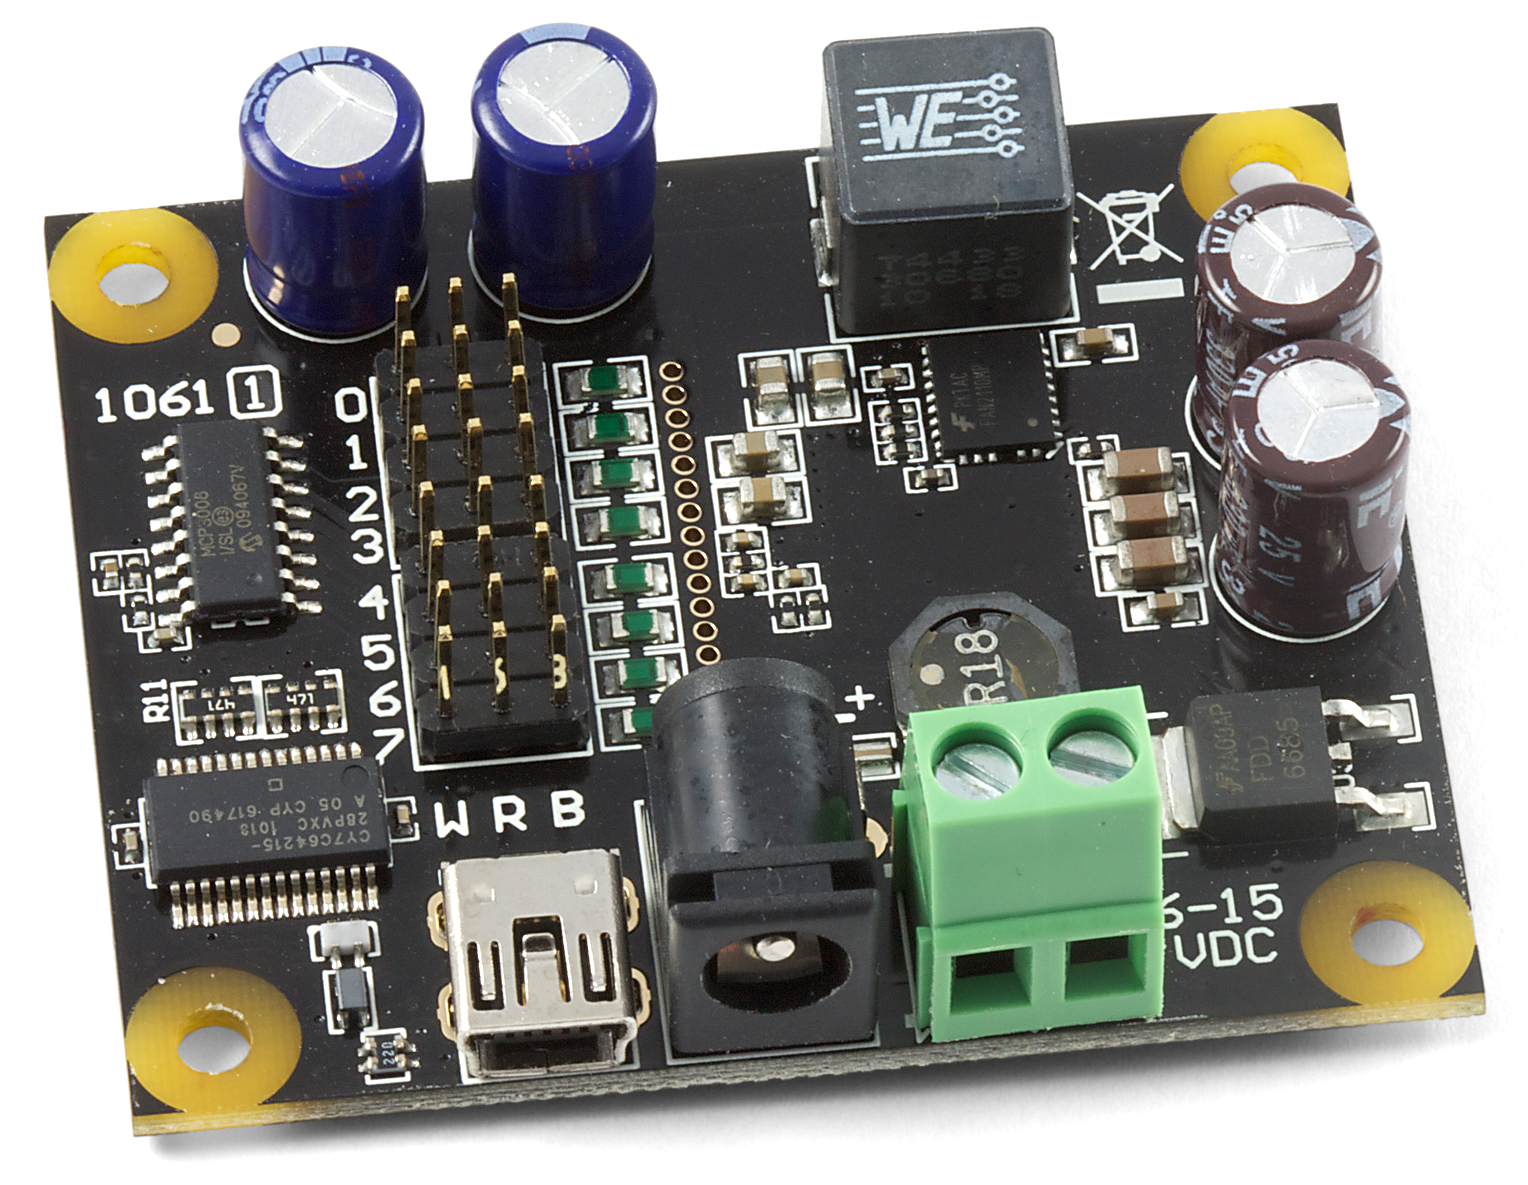
\includegraphics[width=0.4\columnwidth]{ServoController}
   	\vspace{-30pt}
\end{wrapfigure}
pulse width modulation, input from the DreamPlug CPU could be effectively translated into movements of the DC motor, controlling both the speed and direction of the thrusters.

\paragraph{Hall Effect Sensor}

To avoid the high cost of a servo, a Hall effect sensor was set up instead. By placing four magnetic sensors on the worm gear and a transducer which varies based on magnetic field at a fixed location
\begin{wrapfigure}{r}{0.3\columnwidth}
	\vspace{-30pt}
 	\flushright
   	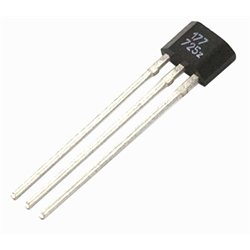
\includegraphics[width=0.3\columnwidth]{HallEffect}
   	\vspace{-30pt}
\end{wrapfigure}
adjacent to it, the degree to which the worm gear has turned can be determined. Checking the orientation of the propulsion thrusters (i.e.~whether they are level, tilted upward/downward, etc.) before powering them on is, of course, crucial in ensuring the AUV travels in the direction intended.

\subsubsection{Input/Output Handling}

Most of I/O handling was sent through an integrated Phidget TextLCD 20x2 and Phidget InterfaceKit 8/8/8 module. This combination module acted as a hub for all components requiring digital or analogue inputs.
\begin{wrapfigure}{r}{0.4\columnwidth}
	\vspace{-30pt}
 	\flushright
   	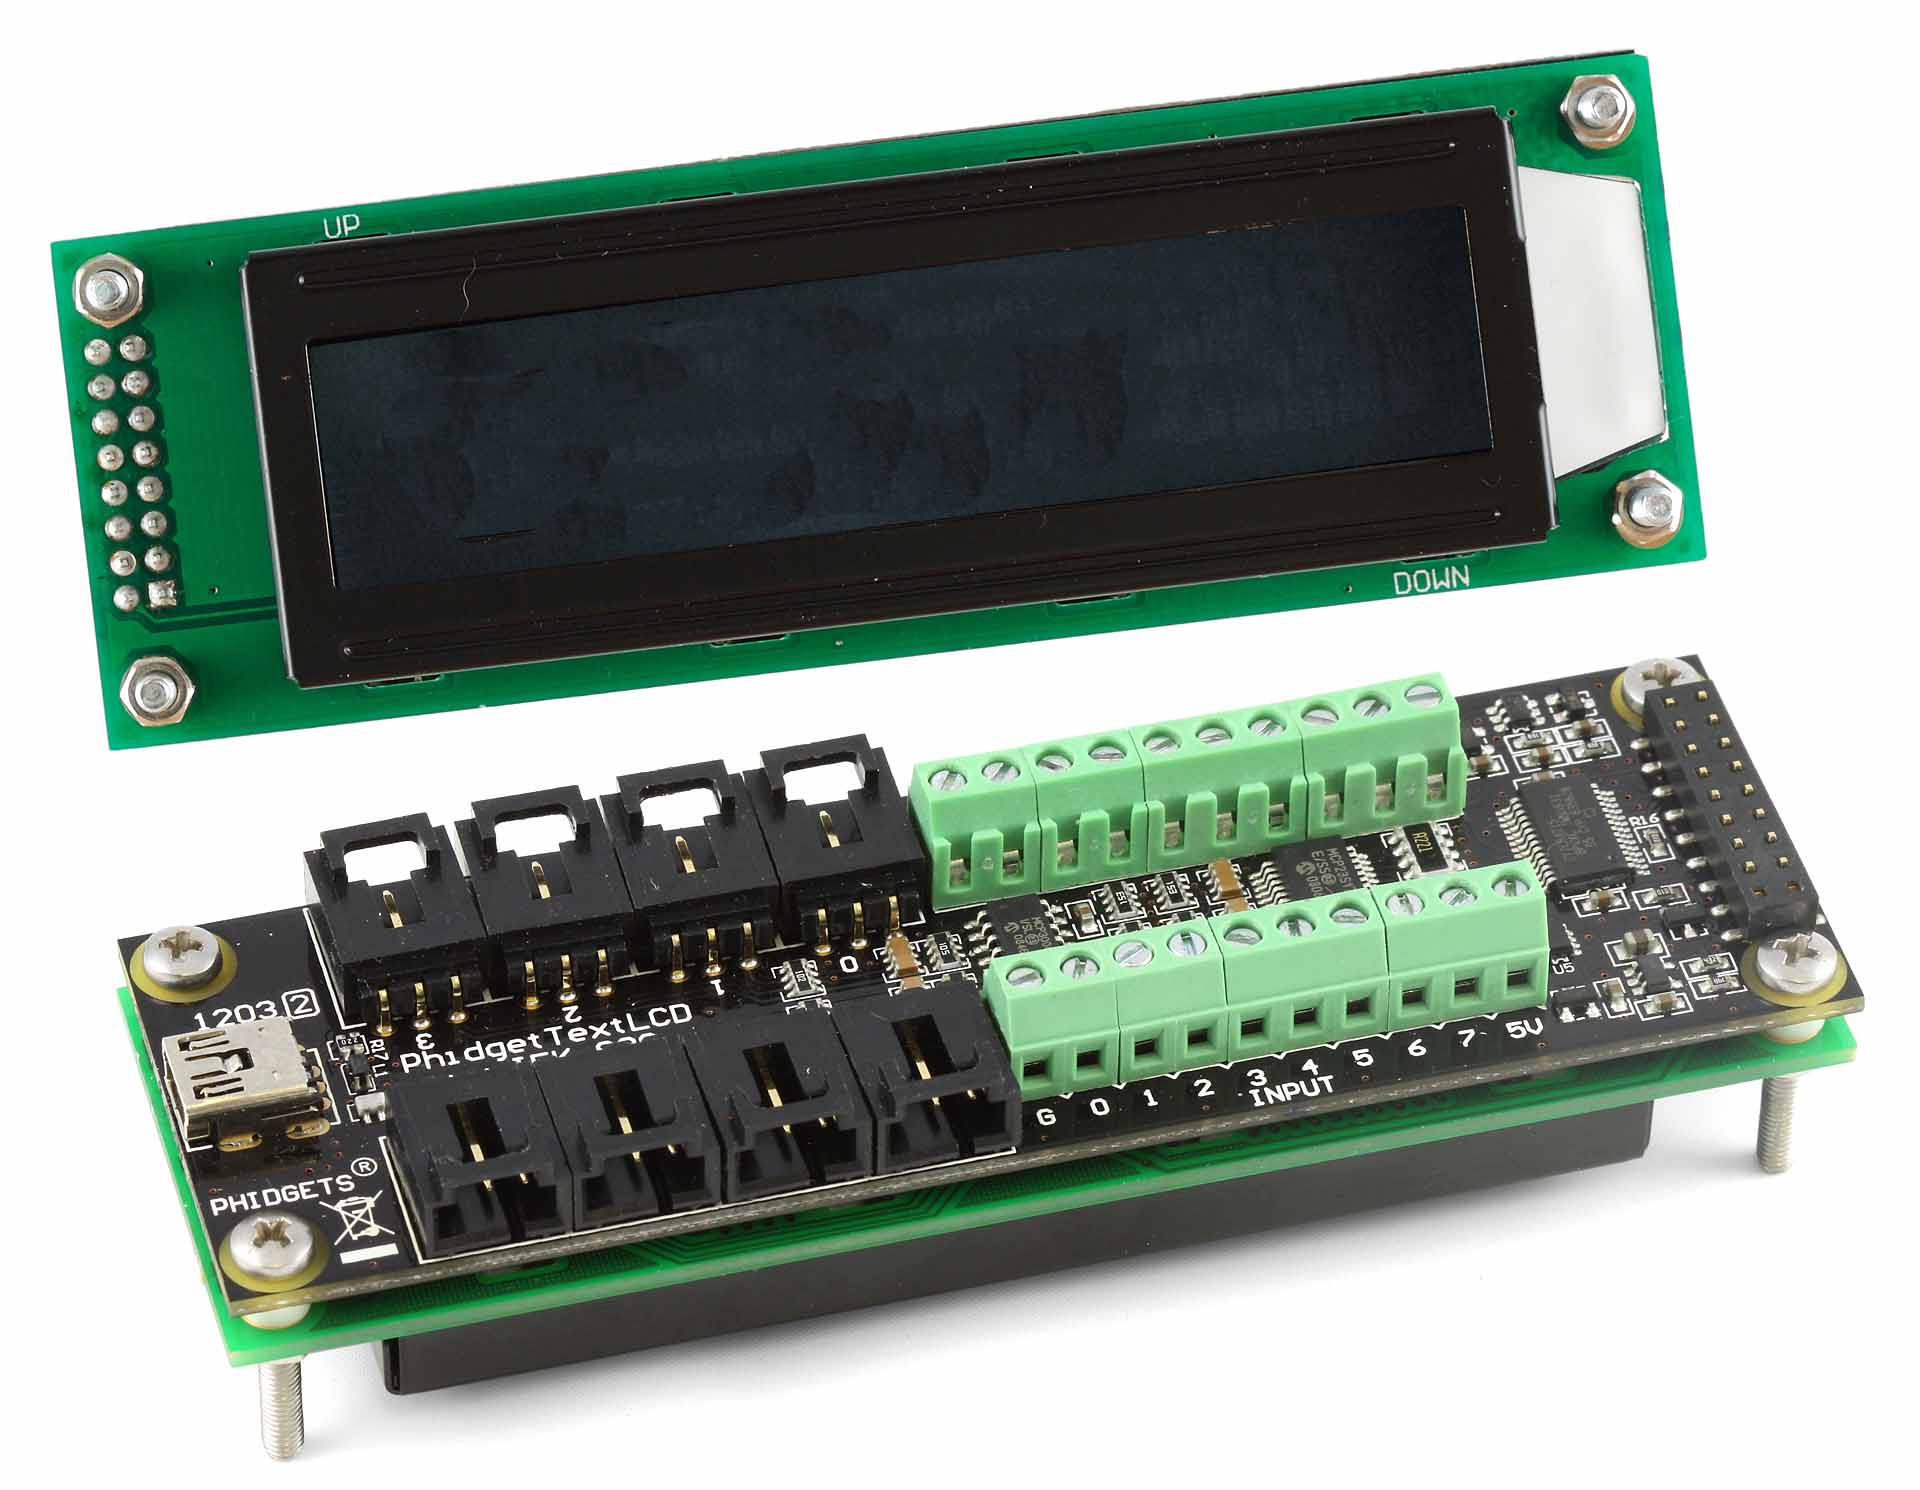
\includegraphics[width=0.4\columnwidth]{LCD}
   	\vspace{-30pt}
\end{wrapfigure}
In addition to communicating signals from the computing core, the display readout on the LCD was used to indicate the AUV's state as it moved through key portions of the code. Coupled with the console data, this provided an efficient method to troubleshoot the robot.

\subsubsection{Spatial Recognition}

The main module used to determine position, orientation, and direction of
\begin{wrapfigure}{r}{0.4\columnwidth}
	\vspace{-30pt}
 	\flushright
   	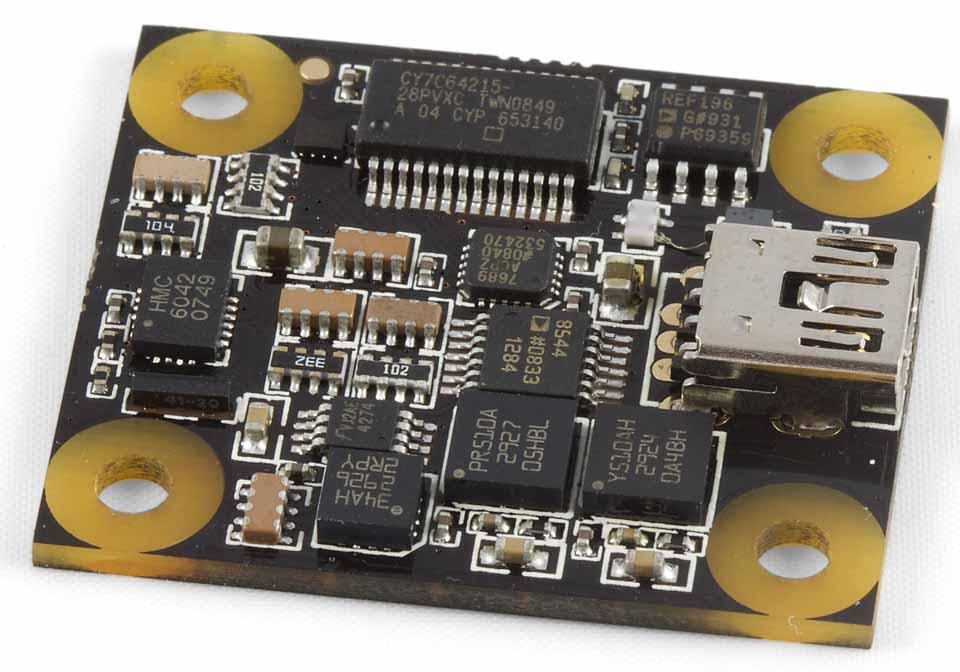
\includegraphics[width=0.4\columnwidth]{Spatial}
   	\vspace{-30pt}
\end{wrapfigure}
the AUV was a Phidget Spatial 3/3/3. This component combines an accelerometer, gyroscope, and compass, all of which would be used in coordination to determine the physical state of the AUV.

\paragraph{Accelerometer}

The accelerometer portion of the module measures both static and dynamic acceleration in all three axes. By integrating the data collected with respect to time, the AUV's speed and position can be determined to a rough degree of accuracy.

\paragraph{Gyroscope}

To ensure that the robot remains in the orientation intended, the gyroscope on the module provides readings of pitch, roll, and yaw underwater. Corrections of orientation will be made with the thrusters in the event that the robot is incorrectly positioned.

\paragraph{Compass}

Although the compass module provided with the Phidget Spatial works quite well, its inconvenient position amidst
\begin{wrapfigure}{r}{0.4\columnwidth}
	\vspace{-30pt}
 	\flushright
   	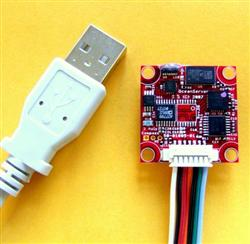
\includegraphics[width=0.4\columnwidth]{Compass}
   	\vspace{-30pt}
\end{wrapfigure}
all of the other electronics on board is liable to cause misreadings in the direction of the AUV. As a result, a second compass, an Ocean Server OS5000-US Solid State Tilt Compensated 3 Axis Digital Compass was installed at the front of the robot, away from the main electronics. The built-in accelerometer (used for tilt compensation) also integrates with the readings from the Phidget Spatial 3/3/3, allowing for more accurate readings with respect to spatial perception.


\subsubsection{Depth Sensor}

To gauge the depth of the AUV, a Honeywell NSCDANN030PAUNV Pressure Sensor
\begin{wrapfigure}{r}{0.3\columnwidth}
	\vspace{-30pt}
 	\flushright
   	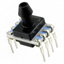
\includegraphics[width=0.3\columnwidth]{Pressure}
   	\vspace{-30pt}
\end{wrapfigure}
was mounted on board the robot. As the resistance of the sensor changes according to pressure, an algorithm can be used to convert the analogue output of the sensor into depth. Because the sensor had to be exposed
to the extremities of the robot in order to take the reading while remaining dry so that the electrical components would be safe, care was taken to ensure that only the sensor portion of the module was exposed, with the rest of the component remaining waterproof. Because depth control is one of the most important aspects of positioning the AUV, this module was critical to the running of the robot.

\section{Software}

Ensuring that the code ran properly was a big challenge, given the very limited testing time the team had. The programming team worked intensely to get the software working as smoothly and as quickly as possible; with only a few members having full knowledge of the API used, this was difficult, but as the team's mission strategy for the AUV this year was not overly complex, the programmers were able to make do with the little time they had.

\subsection{Overview}
\begin{figure}[b!]
   \vspace{-10pt}
   \flushright
      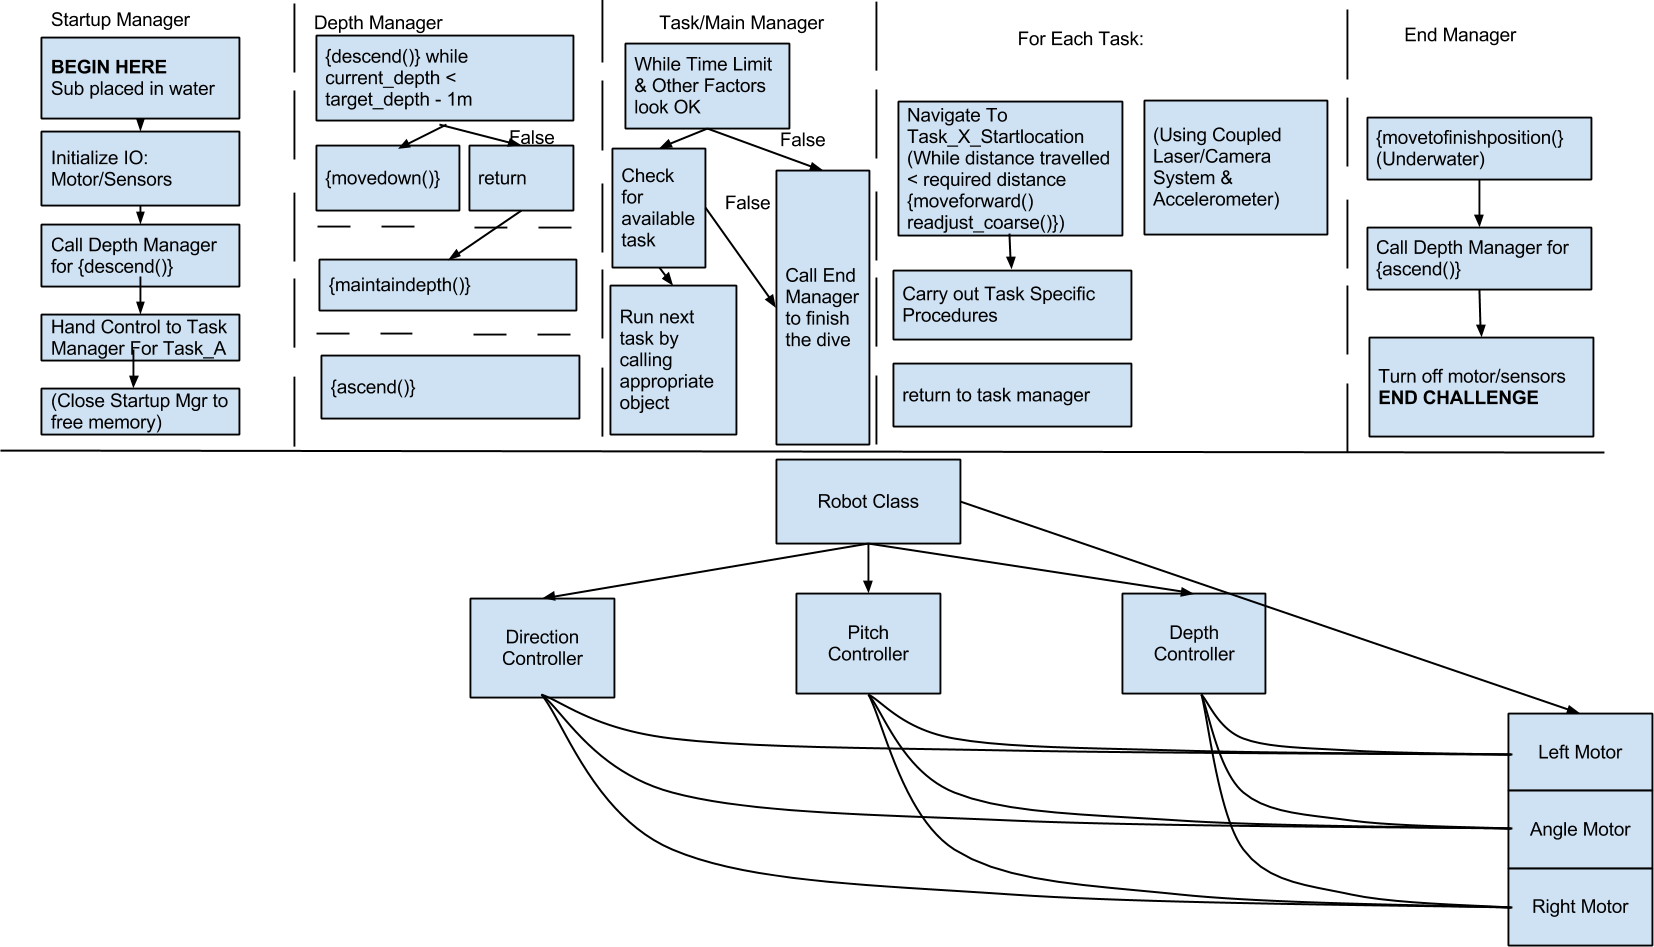
\includegraphics[width=\textwidth]{Flowchart}
      \vspace{-10pt}
\end{figure}

The code for all of the software for the AUV was written in \CPP. In this situation, \CPP\ was the language of choice due to its efficiency, object-oriented nature, and relative simplicity to debug and understand. Most of the programmers on the team come from a Java/Python background, so \CPP\ was a somewhat natural transition into an arguably more powerful language.

All of code was compiled for the DreamPlug computer, running Debian Linux on an ARMv5 architecture. Because the DreamPlug lacked the memory and processing power to compile the code natively in an efficient manner, the team decided to cross-compile their code, storing only the binaries on the DreamPlug system. The source code was written using various text editors, and compiled via command line---because of the numerous platforms and systems that the team members used, a standard IDE was decided against.

The main challenge for the team was to find a way to keep everyone in tune with what was meant to be accomplished, as there were numerous aspects of the software that had to be dealt with. For instance, because each of the sensors relied on different APIs, it was sometimes difficult to debug code that one team member had worked on. Regardless, the programming team found the use of flow charts and other graphical representations of the code very useful.

\subsection{Programming Paradigm}

The programming team decided to take a class-based, top-down approach to the programming. More specifically, each module that was included on the robot would have \newpage\noindent its own separate class, thus allowing a fairly simple means of organizing all of the code.

The general structure of the program was first created using a large flowchart. Then, the methods that needed to be implemented were mapped out and placed onto the diagram. After the team agreed upon which classes, methods, and algorithms to used, each member was assigned a different portion of the code, starting from the broadest tasks (e.g.~instructing the robot to submerge) down to the most fundamental ones (e.g.~measuring and controlling the depth to which the AUV submerges).

\subsection{Input Processing}

As mentioned earlier, each sensor was given its own class, within the class would include methods to read and process data; since the output of each sensor had to be interpreted in a different manner, the team felt that it made most sense to create a common method among all of the sensor classes to read data.

Most of the sensor input went through the Phidget InterfaceKit 8/8/8 module, which served as a hub for both input and output. This was ideal because the InterfaceKit comprised built-in ports on API methods for reading both analogue and digital input (as the sensors on the AUV outputted both types of data), as well as being able to output information on both the LCD display and in the console log.

Filtering the sensor data was perhaps one of the most challenging problems the programming team had to face. As the data generated by the sensors was very noisy, the team was tasked with finding a means to remove these variations and inaccuracies. A basic Kalman filter was developed to clean up the data; however, due to time constraints, the algorithm more closely resembled a moving average filter.

\subsection{Navigation Control}

Controlling the position, orientation, and motion of the robot was the next task, after being able to read the data input from the many sensors on the robot. The team decided to have four fundamental methods that would govern the robot's entire mission: \texttt{move()}, \texttt{goDown()}, \texttt{goUp()}, and \texttt{turn()}. These four methods represent the highest level of abstraction for the AUV; the team worked down from these four methods to create a functioning robot that could complete the tasks originally set out by the mission strategy.

In programming the motion of the motors, one of the major problems that the team faced was the issue of determining how to control the motors as it changed from one position/speed to another so that the transitions could be smoother and more gradual. After some research, the team decided to implement a proportional-integral-derivative controller, which would gradually adjusts the speed of the motor as it approaches a desired setpoint. Despite the fact that implementation of this controller was quite complicated, the team found great success in navigating the AUV smoothly after this was completed.

\section{Conclusion}

It is clear that the St.~George's Robotics Team is not a bringing a AUV into the competition this year that will amaze the audience by completing every challenge in lightning-fast time---far from this, in fact. Nonetheless, the team is quite proud of what has been achieved over the past three years. Myriad challenges and setbacks plagued the team throughout the entire process; despite this however, the team has managed to pull together and put together a robot that accomplishes a great deal, considering the experience of the team.

That being said, the team hopes to be very successful at the 2013 RoboSub Competition. A number of improvements have already been planned for the robot in ensuing years; the team's experience at the competition this year will hopefully only allow even more ideas to transpire and come about.

To the team, this AUV is more than just an AUV; this AUV represents the hard work, the everlasting perseverance, and the undying vision by all of the team members for the past quarter-decade. This AUV represents the product of countless hours of brainstorming, cooperation, and problem solving. More than anything, however, this AUV exemplifies the hopes and dreams that this team has possessed ever since its team members came together. Participating in this competition has been a distant aspiration for so many years; finally realizing this dream has truly been an unforgettable accomplishment.

\section{Acknowledgements}

The utmost respect and appreciation goes to Mr. Andrew Kay, who took many hours out of his busy schedule to tirelessly supervise the team throughout the entire process, providing countless tips and insight to ensure that the robot would function as well as possible at the competition. This robot would not nearly be where it is today were it not for his undying guidance and mentorship.

In addition, because of the team's very limited budget, sponsors make an enormous difference to the success of the robotics program at St.~George's. Many thanks goes to the team's generous sponsors: Whealthfields Lohmann (Hong Kong) Ltd., the St.~George's Parents' Association, and Stollco Industries. Their contributions have truly helped made the team's participation in the 2013 RoboSub Competition possible.

\end{document}
